\documentclass{beamer}

% fonts
\usepackage[utf8]{inputenc}
\usepackage[francais]{babel}

% asm
\usepackage{amsmath}
\usepackage{amssymb}
\usepackage{amsthm}

% diagrams
\usepackage{tikz}
\usetikzlibrary{matrix}
\usetikzlibrary{positioning}

% titlepage
\title{Lattice Reduction Techniques\\To Attack RSA}
\author{David Wong}
\institute{University of Bordeaux}
\date{March 2015}
\setbeamercolor*{title}{fg=white}
\setbeamercolor*{author}{fg=white}
\setbeamercolor*{institute}{fg=white}
\setbeamercolor*{date}{fg=white}

%
\begin{document}

% TITLE
\fontsize{16pt}{15.2}\selectfont
\usebackgroundtemplate{
\includegraphics[width=\paperwidth,height=\paperheight]{img/blurry.jpg}} 
\begin{frame}
\titlepage
\end{frame}

% RSA
\fontsize{90pt}{15.2}\selectfont
\usebackgroundtemplate{
\includegraphics[width=\paperwidth,height=\paperheight]{img/blurry2.jpg}}
\begin{frame}
\begin{center}
\textbf{RSA?}
\end{center}
\end{frame}

% ENCRYPT/DECRYPT
\fontsize{14pt}{15.2}\selectfont
\usebackgroundtemplate{}
\begin{frame}
$(e, N)$ is the \textbf{public key}, 
$(d, N)$ is the \textbf{private key}.\\

\pause

\vspace{1cm} To \textbf{encrypt} a message $m$, with $m < N$ we just do:
\[ c = m^e \pmod{N} \]
\pause
And to \textbf{decrypt}:
\[ m = c^d \pmod{N} \]
\end{frame}

\begin{frame}
To generate these keys, we first generate \textbf{two primes} $p$ and $q$ such that:
\[ N = p \times q \]
\pause
Use $p$ and $q$ to generate the pair \textbf{private key/public key} $(d,e)$.
\end{frame}

% ATTACKS?
\fontsize{90pt}{15.2}\selectfont
\usebackgroundtemplate{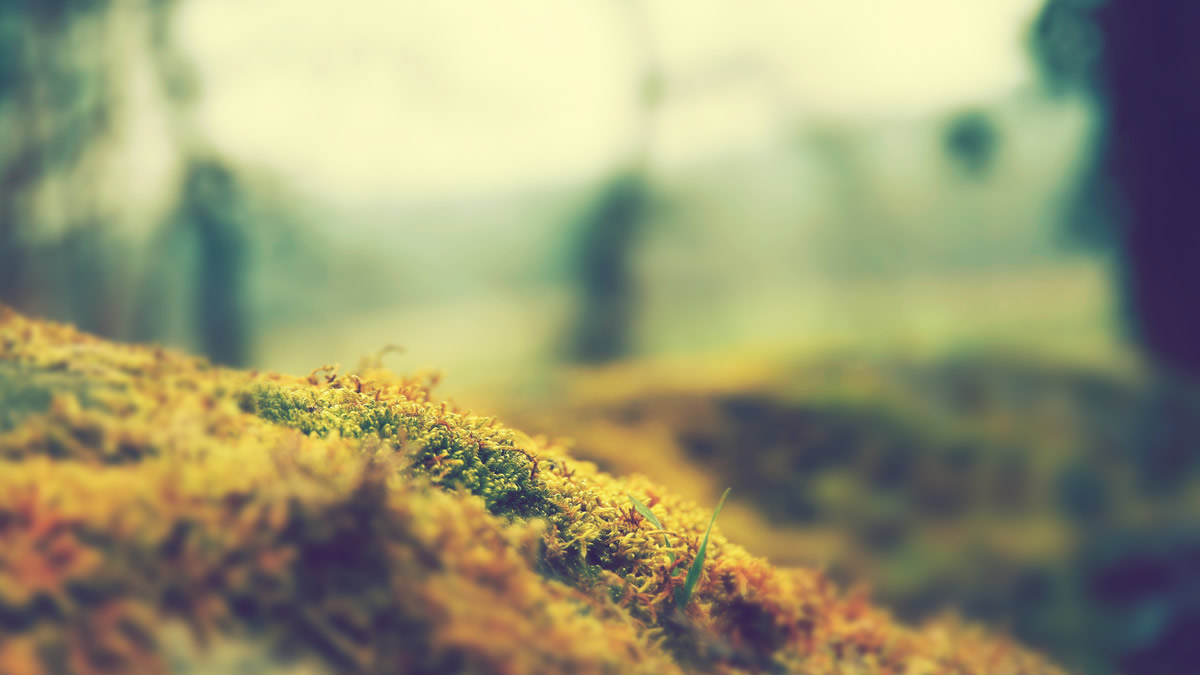
\includegraphics[width=\paperwidth,height=\paperheight]{img/blurry3.jpg}}
\begin{frame}
\begin{center}

\textbf{ATTACKS?}
\end{center}
\end{frame}

%
\fontsize{14pt}{15.2}\selectfont
\usebackgroundtemplate{}
\begin{frame}

On the implementation or on the mathematics.\\\vspace{1cm}
\pause
 \textbf{Model}:

\begin{itemize}
	\item{Recover the plaintext $m^e = c \pmod{N}$}
	\item{Recover the private key $d$}
\end{itemize}
\vspace{1cm}
\pause
\textbf{Relaxed model}:
\pause
\begin{itemize}
	\item{We know a part of the message}
	\item{We know an approximation of one of the prime}
	\item{The private exponent is too small}
\end{itemize}
\end{frame}

% LATTICE
\fontsize{90pt}{15.2}\selectfont
\usebackgroundtemplate{
\includegraphics[width=\paperwidth,height=\paperheight]{img/blurry4.jpg}}
\begin{frame}
\begin{center}

\textbf{LATTICE?}
\end{center}
\end{frame}

% VECTOR SPACE
\fontsize{16pt}{15.2}\selectfont
\usebackgroundtemplate{}
\begin{frame}

A bit like a \textbf{vector space}.\vspace{1cm}

\begin{tikzpicture}[scale=.45]
\draw [lightgray] [<->] (0,5) -- (10,5);
\draw [lightgray] [<->] (5,10) -- (5,0);
\draw [thick,purple] [->] (5,5) -- (6, 8);
\draw [thick,purple] [->] (5,5) -- (6, 6);

\draw [thick,black] [->] (11,5) -- (12,5);

\draw [lightgray] [<->] (13,5) -- (23,5);
\draw [lightgray] [<->] (18,10) -- (18,0);
%\path [fill=purple] (18,5) to (20.5,10) to (23,10) to (18,5);
\path [fill=purple] (15.5,0) to (20.5,10) to (23,10) to (13,0);
\end{tikzpicture}\\
\end{frame}


% COPPERSMITH
\fontsize{35pt}{15.2}\selectfont
\usebackgroundtemplate{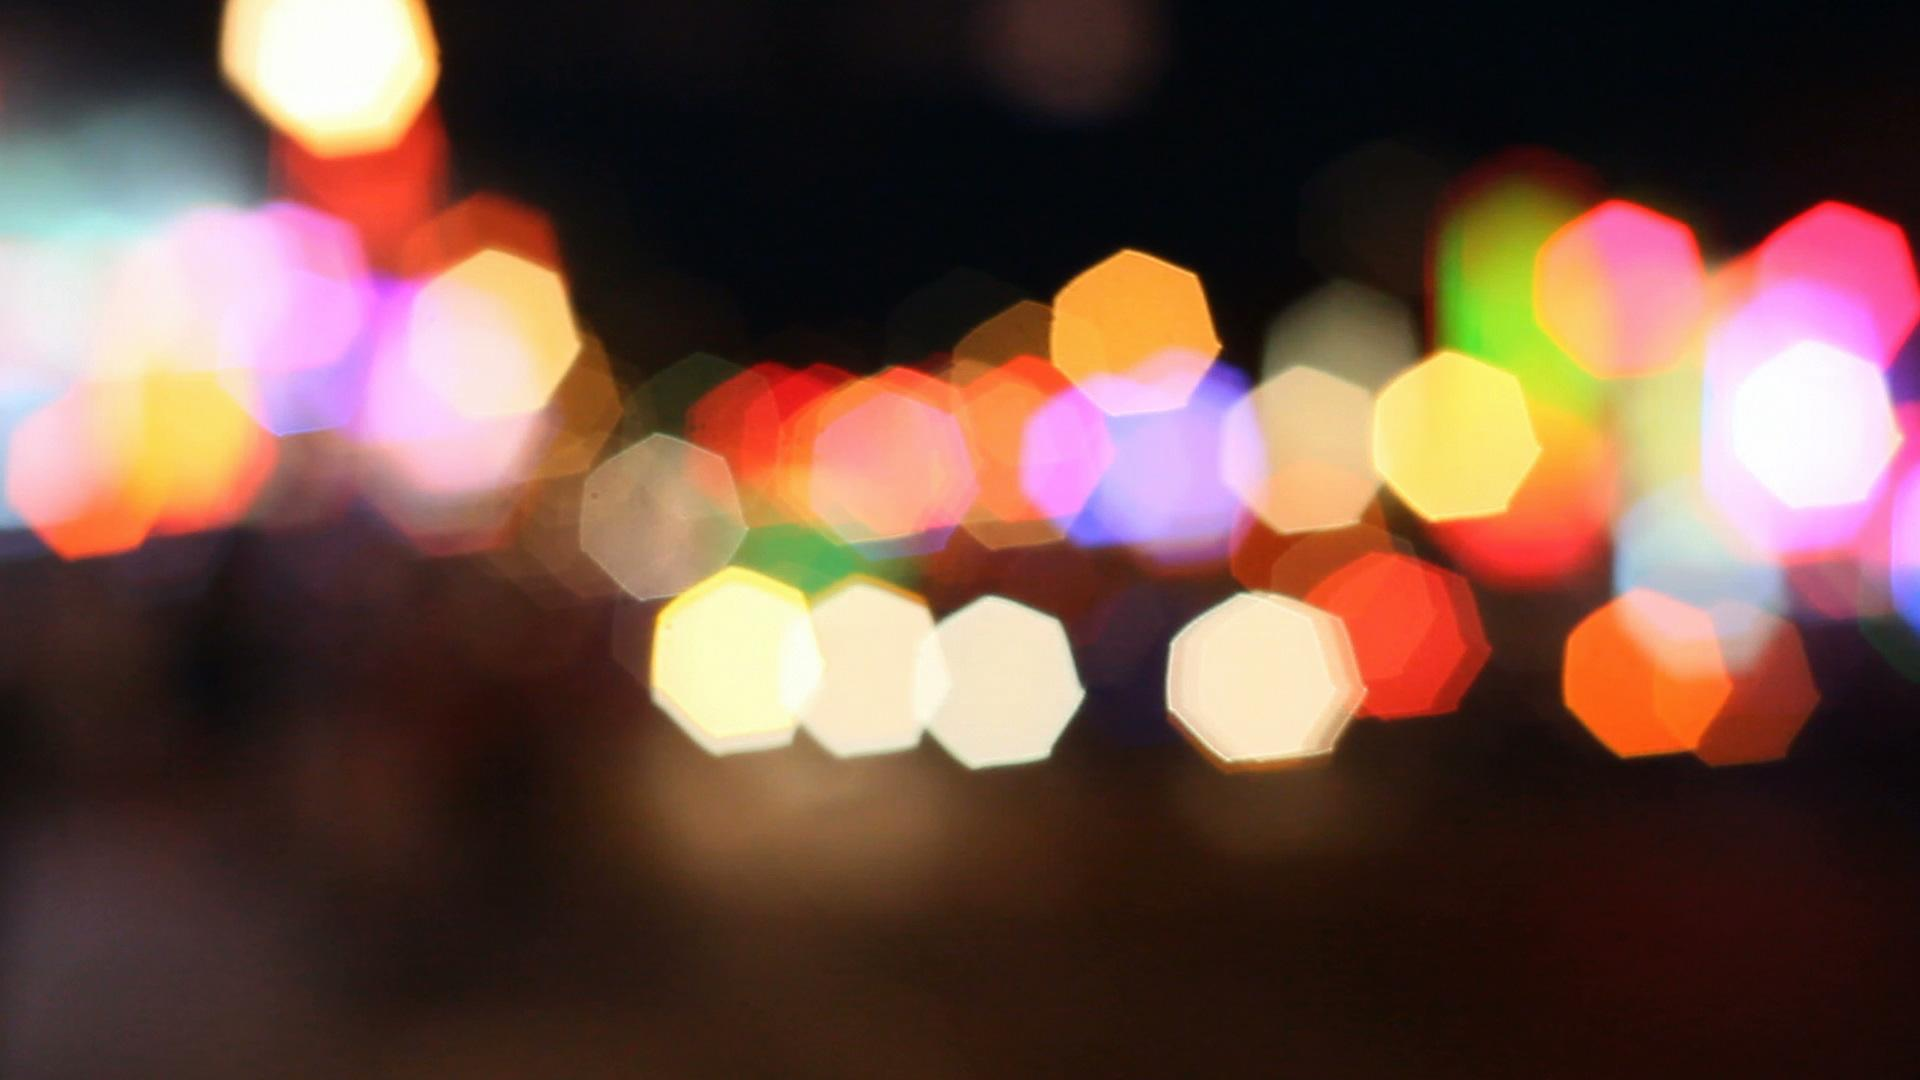
\includegraphics[width=\paperwidth,height=\paperheight]{img/blurry5.jpg}}
\begin{frame}
\begin{center}

\textbf{COPPERSMITH?}
\end{center}
\end{frame}

% VECTOR SPACE
\fontsize{16pt}{15.2}\selectfont
\usebackgroundtemplate{}


% BONEH-DURFEE
\fontsize{90pt}{15.2}\selectfont
\usebackgroundtemplate{
\includegraphics[width=\paperwidth,height=\paperheight]{img/blurry6.jpg}}
\begin{frame}
\begin{center}

\textbf{BONEH-DURFEE?}
\end{center}
\end{frame}

% VECTOR SPACE
\fontsize{16pt}{15.2}\selectfont
\usebackgroundtemplate{}
%
\end{document}